\documentclass[12pt]{article}
\usepackage[english]{babel}
\usepackage{natbib}
\usepackage{url}
\usepackage[utf8]{inputenc}
\usepackage{amsmath}
\usepackage{amssymb}
\usepackage{graphicx}
\usepackage{parskip}
\usepackage{fancyhdr}
\usepackage{vmargin}
\usepackage{booktabs}
\usepackage[table,xcdraw,dvipsnames]{xcolor}
\usepackage{listings}
\usepackage{tabularx}
\usepackage{caption} 
\usepackage{float}
\usepackage{longtable}
\usepackage{array}
\usepackage{caption}
\usepackage{subcaption}


\setmarginsrb{3 cm}{1 cm}{3 cm}{1 cm}{1 cm}{1.5 cm}{1 cm}{1.5 cm}

\newcolumntype{L}[1]{>{\raggedright\let\newline\\\arraybackslash\hspace{0pt}}m{#1}}
\newcolumntype{C}[1]{>{\centering\let\newline\\\arraybackslash\hspace{0pt}}m{#1}}
\newcolumntype{R}[1]{>{\raggedleft\let\newline\\\arraybackslash\hspace{0pt}}m{#1}}

\usepackage{natbib}

\title{Assignment \#3 - Population Testing}
\date{\today}

\makeatletter
\let\thetitle\@title
\let\thesubtitle\@subtitle
\let\theauthor\@author
\let\thedate\@date
\makeatother

\pagestyle{plain}

\captionsetup[table]{skip=5pt}


\begin{document}

%%%%%%%%%%%%%%%%%%%%%%%%%%%%%%%%%%%%%%%%%%%%%%%%%%%%%%%%%%%%%%%%%%%%%%%%%%%%%%%%%%%%%%%%%

\begin{titlepage}
	\centering
    \textsc{\LARGE University of Coimbra}\\[1.0 cm]
	\textsc{\large Doctoral Program in Information Science and Technology}\\[0.5 cm]
    \textsc{\large Statistics}\\[5 cm]
	\rule{\linewidth}{0.2 mm} \\[0.4 cm]
	{ \LARGE \bfseries \thetitle}\\ [0.2 cm]
    \rule{\linewidth}{0.2 mm} \\[3 cm]
    
    \textsc{Joaquim Pedro Bento Gonçalves Pratas Leitão - 2011150072}\\[5 cm]
	
	{\large \thedate}\\[2 cm]
 
	\vfill
	
\end{titlepage}

%%%%%%%%%%%%%%%%%%%%%%%%%%%%%%%%%%%%%%%%%%%%%%%%%%%%%%%%%%%%%%%%%%%%%%%%%%%%%%%%%%%%%%%%%

\section{Introduction}
\label{introduction}

The current document is framed in the scope of the third assignment of the Statistics course, taught for the Doctoral Program in Information Science and Technology at the University of Coimbra, during the academic year of 2016/2017.

The current assignment focus on parametric and non-parametric significance tests with respect to the average of a given population of which a sample was observed and collected.

The data collected for this assignment through a survey of fast-food consumption habits in England was used in this study, and the opinions of $344$ consumers who reported buying fast food regularly were recorded. The supplied dataset contains the following variables:

\begin{itemize}
	\item Average number of weekly fast-food purchases in the last month.
	
	\item Age of the reporting person, divided in five classes: \textbf{1} for people with ages between 15 and 17, \textbf{2} for 18-24, \textbf{3} for 25-35, \textbf{4} for 36-54 and \textbf{5} for 55-70.

	\item Genre of the reporting person.
	
	\item Socio-economic level of the reporting person, divided in three classes: \textbf{1} for low, \textbf{2} for medium and \textbf{3} for high.
	
	\item Educational qualifications of the reporting person, divided in four classes: \textbf{1} for high school level, \textbf{2} for technical course, \textbf{3} for B.Sc degree and \textbf{4} for MSc or PhD.
\end{itemize}

As already mentioned, the main focus and goal of the current assignment was on the application of adequate parametric and non-parametric significance tests to the collected and observed samples, in order to withdraw conclusions with respect to the entire population under study.

The main variable under analysis is the average number of weekly fast-food purchases, and the three tests proposed for the current assignment relate this variable with some of the remaining collected variables: In the first two tests fast-food purchases are related with the genre of the inquired people and in the final test an analysis of fast-food purchases by age is performed.

As required, all tests were performed with a significance level of $0.05$. In addition, all tests documented in this report were performed using the \emph{R}\footnote{\url{https://www.r-project.org/}} software environment.

In the remainder of this document the tests proposed in the current assignment will be covered: In section \ref{genre_tests} the first two tests are presented and discussed, while section \ref{age_tests} is reserved for the third test.

\section{Fast-Food Purchases by Genre}
\label{genre_tests}

In the current section the two proposed tests to relate fast-food purchases with the survey respondents' genre are covered.

\subsection{Purchases by Women}

As a starting point it was intended to analyse the average fast-food purchases made by women, in order to determine whether or not this average value (in the previous month) is significantly higher than a given value, 2.5 in our scenario.

\subsubsection{Approach to the Problem}

Taking into account that only one variable was being analysed at this point (corresponding to a subset of the collected sample) we are faced with a test for the average of a population, which may or may not be parametric. Therefore, a \emph{Student's T-Test} (T-Test) appears as the most promising test, provided its assumptions can be met.

Since the T-Test assumes the random variable in question follows a normal distribution, the initial step in this problem will be determining whether or not the variable of interest (in this case, the average fast-food purchases made in the last month) follows a normal distribution.

To this end, a \emph{Shapiro-Wilk} test for normality in the variable of interest was performed. A \emph{p-value} of $7.191026e^{-12}$ was registered in this test. As this \emph{p-value} is considerably smaller than the required significance level, the test's null hypothesis (stating that the variable under analysis follows a normal distribution) is rejected, at the significance level of $0.05$.

These results are further supported by the histogram of the average fast-food purchases by women, presented in figure \ref{histogram_women_purchases}.

\begin{figure}[H]
	\centering
	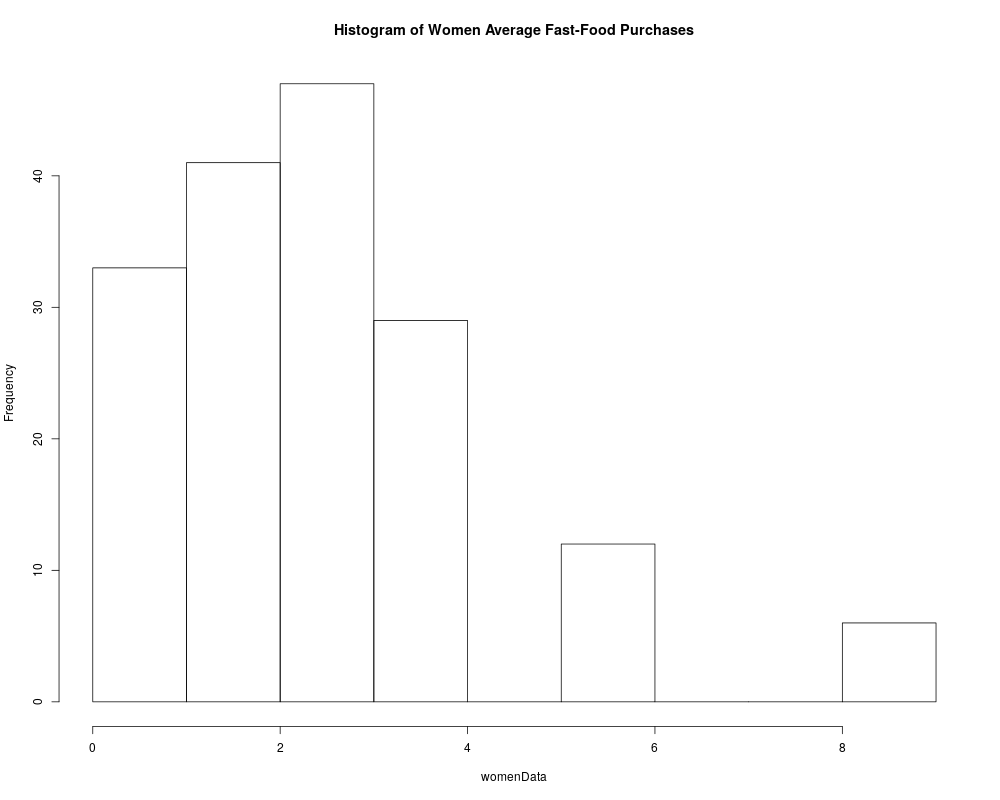
\includegraphics[scale=0.28]{images/Histogram_WomenData.png}
	\caption{Histogram of fast-food purchases by women.}
	\label{histogram_women_purchases}
\end{figure}

A practical result of the application of the \emph{Shapiro-Wilk} test for the fast-food purchases by women implies that this variable cannot be accepted to follow a normal distribution.

Even though normality cannot be assured for our study variable, the T-Test  can still be applied to this variable, provided its number of observations is higher than $30$. In this case we obtain an approximate \emph{p-value} for the test. Considering that a total of $168$ women answered the survey, the T-Test can still be applied to the fast-food purchases made by women (as $168 > 30$).

As a result, the following hypothesis were considered in the T-Test:

$$ H0: \: m_{X} = 2.5 \: \: \: vs \: \: \: H1: m_{X} > 2.5$$

where \emph{X="Average number of weekly fast-food purchases made by women in the last month"}.

For this test an approximate \emph{p-value} of $0.2779$ was registered. As this value is considerably higher than the required significance level ($0.05$) the null hypothesis is accepted, at this significance level. Such hypothesis states that the average number of weekly fast-food purchases made by women in the last month is 2.5.

Based on what was presented in this subsection and on the results of the performed hypothesis tests, the main conclusion to be withdrawn at this point is that it cannot be concluded that the average number of weekly fast-food purchases made by women in the last month is significantly higher than 2.5.

\subsubsection{R Implementation}

In listing \ref{analysewomenfastfood} the \emph{R} implementation of the detailed approach is presented. This listing contains only the core commands developed in the course of this work; as such, additional commands can be found in the \emph{R} scripts provided with this report (namely commands used for debugging or for presenting the obtained results to the user).

\lstset{language=R,extendedchars=true,frame=single,
	caption={AnaylseWomenFastFood.R},label={analysewomenfastfood},tabsize=2,keywordstyle=\color{RoyalBlue},commentstyle=\color{YellowGreen},stringstyle=\color{ForestGreen},showstringspaces=false}
\begin{lstlisting}
AnaylseWomenFastFood <- function(dataset) {
  # Analyses the average number of weekly purchases made by
  # women in the last month and determines if its average
  # level is significantly higher than 2.5 .
  #
  # Args:
  #   dataset: A dataframe with the observed data.
  #
  
  significanceLevel = 0.05
  confidenceLevel = 1 - significanceLevel

  # Filter data: Only collect information for the women and
  # then select only the "Compras" field
  womenData <- subset(dataset, Sexo=='2')
  womenData <- womenData$Compras

  # Just plot the histogram of the desired data
  png('images/Histogram_WomenData.png', width=1000,
      height=800)
  hist(womenData,
       main='Histogram of Women Average Fast-Food Purchases')

  # Test for normality with Shapiro-Wilk
  shapiroResult <- shapiro.test(womenData)
  
  # Compare the p-value (shapiroResult$p.value) with the
  # significance level.
  
  # The obtained p-value for the Shapiro-Wilk Test is very
  # small (7.191e-12) therefore, at the significance level
  # of 0.05, we reject the null hypothesis stating that the
  # observed data follows a normal distribution.
  # Nevertheless, since the length of the observed data is
  # considerably higher than 30 (168 > 30) we can still
  # apply the T-Test for the mean of a population and
  # obtain an approximate p-value.


  # In the T-Test for the mean of a population we are
  # considering the following hypothesis:
  #     H0: m = 2.5
  #     H1: m > 2.5
  tResult <- t.test(womenData, alternative='greater',
                    mu=2.5, paired=FALSE,
                    conf.level=confidenceLevel)
  
  # Compare the p-value (tResult$p.value) with the
  # significance level.

  # We obtain an approximate p-value of 0.2779 for the
  # T-Test. For a significance level of alfa = 0.05 we
  # verify that p-value > alfa. Therefore, and at the
  # referred significance level, we accept the null
  # hypothesis stating that m = 2.5

  dev.off()
}
\end{lstlisting}


\subsection{Purchases by Women and Men}

Extending the analysis performed in the previous subsection, the second proposed exercise intended to compare the average fast-food purchases by both women and men, in order to determine if the average purchases by women is significantly higher than the ones made by men.

\subsubsection{Approach to the Problem}

In such an exercise it is intended to compare the means of two populations: The average purchases by women and by men. Therefore, a \emph{Student's T-Test} (T-Test) appears as the most promising significance test to be performed. Similarly to what was done in the previous subsection, prior to the execution of the test, its assumptions must be met.

When comparing the means of two populations the T-Test has two possible formulations, one applied when the collected samples are independent, and another when in the presence of paired samples. As purchases by women and men have no relation between then, therefore there is no pairing between collected samples of the two populations, in the current exercise a T-Test for independent samples is considered.

Besides assuming the independence of the corresponding random variables, this T-Test also assumes the normality of both variables. When one of the variables (or both) does not follow a normal distribution the test can still be applied, provided a high number of samples is collected for both variables (higher than 30). In this scenario, an approximated \emph{p-value} is obtained.

To this end, the analysis in this exercise started by performing a \emph{Shapiro-Wilk} test for normality in both variables (purchases made by women and by men). Since the \emph{Shapiro-Wilk} test was performed in the previous exercise for the average fast-food purchases made by women, in the current exercise this test was only performed for the average fast-food purchases made by men.

The normality test registered a \emph{p-value} of $2.515e^{-10}$, which is considerably smaller than the required significance level. As a result, the test's null hypothesis (stating that the variable under analysis follows a normal distribution) is rejected, at the significance level of $0.05$. This result is further supported by the histogram of the average fast-food purchases by men, presented in figure \ref{histogram_men_purchases}.

\begin{figure}[H]
	\centering
	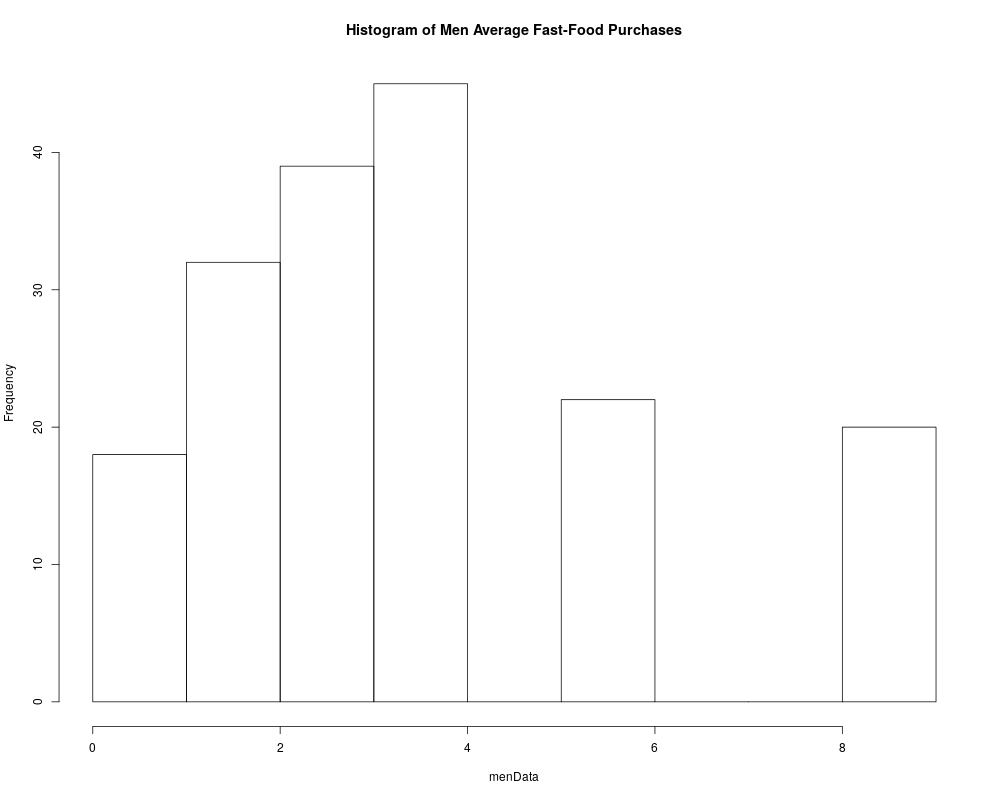
\includegraphics[scale=0.28]{images/Histogram_MenData.png}
	\caption{Histogram of fast-food purchases by men.}
	\label{histogram_men_purchases}
\end{figure}

Since both variables being considered in this exercise registered considerably small \emph{p-values} in their normality tests, at the required significance level, their normality cannot be accepted; however, taking into account that the number of collected samples for each variable is considerably higher ($168$ for women and $176$ for men, which are both higher than $30$), the T-Test can still be applied and an approximate \emph{p-value} will be obtained.

As a result, the following hypothesis were considered in the T-Test:

$$ H0: \: m_{X} - m_{Y} = 0 \: \: \: vs \: \: \: H1: m_{X} - m_{Y} > 0$$

where \emph{X="Average number of fast-food purchases per week made by women in the last month"} and \emph{Y="Average number of fast-food purchases per week made by men in the last month"}.

The T-Test for independent samples considers two distinct test statistics to be computed, depending on the equality (or not) of the variances of the random variables. Therefore, the next step to be performed in this exercise is to analyse the variance equality between the two considered variables. Such a task is accomplished by performing the \emph{Levene's Test} for variance equality. In this test, a \emph{p-value} of $0.002105$ was registered. Since this value is considerably smaller than the required significance level, the null hypothesis is rejected and the variances must be considered different, at the required significance level.

In this scenario (independent samples with different variances) the T-Test with Welch modification is performed. An approximate \emph{p-value} of $0.999994$ was registered. As this value is considerably higher than the required significance level, the null hypothesis of this test is accepted (again, at the required significance level).

Based on what was presented in the current subsection, at the significance level of $0.05$, one can state that the  average purchases made by women and men in the previous month are not significantly different (and, therefore, the purchases made by women are not significantly higher than the ones made by men).

\subsubsection{R Implementation}

In listing \ref{analysewomenmenfastfood} the \emph{R} implementation of the detailed approach is presented. Similarly to the previous problem, this listing contains only the core commands developed in the course of this work. Additional commands can be found in the \emph{R} scripts provided with this report.

\lstset{language=R,extendedchars=true,frame=single,
	caption={AnaylseWomenMenFastFood.R},label={analysewomenmenfastfood},tabsize=2,keywordstyle=\color{RoyalBlue},commentstyle=\color{YellowGreen},stringstyle=\color{ForestGreen},showstringspaces=false}
\begin{lstlisting}
AnalyseWomenMenFastFood <- function(dataset) {
  # Analyses the average number of weekly purchases made by
  # women and men in the last month and determines if the
  # average level of women purchases is significantly higher
  # than that of the man.
  #
  # Args:
  #   dataset: A dataframe with the observed data.

  library(car)

  significanceLevel = 0.05
  confidenceLevel = 1 - significanceLevel

  # X: "Average number of fast-food purchases per week made
  #     by women in the last month"
  # Y: "Average number of fast-food purchases per week made
  #     by men in the last month"
  #
  # We want to test H0: mx - my = 0 vs H1: mx - my > 0

  # Filter Women data
  womenData <- subset(dataset, Sexo=='2')
  womenData <- womenData$Compras

  # Filter Men data
  menData <- subset(dataset, Sexo=='1')
  menData <- menData$Compras

  # Just plot the histogram of the desired data
  png('images/Histogram_MenData.png', width=1000, height=800)
  hist(menData,
       main='Histogram of Men Average Fast-Food Purchases')

  # Test X and Y for normality
  # In the previous exercise we have already tested X for
  # normality and, according to the Shapiro-Wilk Test at a
  # significance level of 0.05 we reject the null
  # hypothesis stating that the data follows a normal
  # distribution.
  # Therefore, in this exercise, we just need to perform
  # the same test for Y.
  shapiroResult <- shapiro.test(menData)

  # Compare the p-value (shapiroResult$p.value) with the
  # significance level.

  # The Shapiro-Wilk test for normality for the Y variable
  # returns a p-value of 2.515e-10. Indeed, this is a very
  # small value which, at the significance level of 0.05,
  # makes us reject the null hyphtoesis stating that the data
  # follows a normal distribution.
  #
  # Even though both X and Y variables do not follow a normal
  # distribution, since the length of the observed data for
  # both variables is considerably higher than 30 (168 for
  # women and 176 for men) we can still aplly the T-Test
  # for the mean difference of two populations, obtaining
  # an approximate p-value.
  #
  # Furthermore, because X and Y are independent, we will be
  # applying the T-Test for the mean difference of two
  # independent populations. The next step in this exercise
  # is to evaluate whether or not the variances of X and Y
  # are equal. Such evaluation can be achieved by performing
  # the Levene's Test.

  # Perform the Levene's Test for Variance Equality
  temp <- data.frame(Compras=dataset$Compras,
                     Sexo=factor(dataset$Sexo))
  leveneResult <-leveneTest(Compras ~ Sexo, data=temp)

  # Get p-value from Levene Test
  leveneP <- (leveneResult$`Pr(>F)`)[1]

  if (leveneP <= significanceLevel) {
   cat('\n     Result: Variances of X and Y are different\n')
   varianceEquality = FALSE
  } else {
   cat('\n     Result: Variances of X and Y are equal\n')
   varianceEquality = TRUE
  }

  # Perform T-Test according to the Levene's Test results
  #     H0: mx - my = 0
  #     H1: mx - my > 0
  tResult <- t.test(womenData, menData,
                    alternative='greater',
                    mu=0, paired=FALSE,
                    var.equal=varianceEquality,
                    conf.level=0.95)


  # Compare the p-value (tResult$p.value) with the
  # significance level.
  
  dev.off()
}
\end{lstlisting}

\section{Fast-Food Purchases by Age}
\label{age_tests}

In the final exercise average fast-food purchases are intended to be analysed according to the consumers' age group, in order to determine if a significant difference is registered between the five age groups considered.

\subsubsection{Approach to the Problem}

When comparing two or more groups with respect to the location, \emph{ANOVA} appears as the parametric test of choice, with \emph{Kruskal-Wallis} being its non-parametric equivalent.

In order to be applied, ANOVA assumes the normality of each group being considered and the homogeneity of their variances (that is, the variances of the groups must be equal). Similarly to the approach carried out in previous exercises, the first step to compare the average fast-food purchases by consumers' age group is to determine whether or not each group follows a normal distribution.

To accomplish this, observed data for each group is collected and the \emph{Shapiro-Wilk} normality test is performed on each of these groups. In the current work, the normality test was first applied to age group number \textbf{2} (for people with ages ranging from 18 to 24 years old), registering a \emph{p-value} of $0.0003072$. As this is considerably smaller than the required significance level, the fast-food purchases for people in the second group cannot be accepted to follow a normal distribution, at the significance level of $0.05$.

As a result, the first assumption of the ANOVA cannot be met (the normality of each group) and therefore this parametric test is not applicable to the collected data. Its non-parametric alternative, the \emph{Kruskal-Wallis} is thus applied to our collected data.

When applying the \emph{Kruskal-Wallis} test for mean equality, a \emph{p-value} of $4.751e^-{06}$ was registered. As this is considerably smaller than the required significance level the null hypothesis stating that all means are equal is rejected. Therefore, at the significance level of $0.05$, fast-food purchases differ according to the consumers' age group.

\subsubsection{R Implementation}

In listings \ref{analyseagegroupfastfood} and \ref{testifanova} the \emph{R} implementation of the detailed approach is presented. Similarly to the previous problem, these listing contain only the core commands developed in the course of this work. Additional commands can be found in the \emph{R} scripts provided with this report.

\lstset{language=R,extendedchars=true,frame=single,
	caption={AnalyseAgeGroupFastFood.R},label={analyseagegroupfastfood},tabsize=2,keywordstyle=\color{RoyalBlue},commentstyle=\color{YellowGreen},stringstyle=\color{ForestGreen},showstringspaces=false}
\begin{lstlisting}
AnalyseAgeGroupFastFood <- function(dataset) {
  # Analyses the average weekly number of purchases in the
  # last month and determines if it is significantly
  # different according to the age group of the people that
  # answered the survey.
  #
  # Args:
  #   dataset: A dataframe with the observed data.
  #

  # When comparing two or more groups with respect to the
  # location, ANOVA appears as the parametric test of choice,
  # with Kruskal-Wallis being its non-parametric equivalent.
  # Therefore, in this approach, we will start by checking
  # whether or not the ANOVA can be applied. If its
  # assumptions cannot be verified then we will move on to
  # the Kruskal-Wallis test.

  # Start by getting all the age groups
  ageGroups <- unique(dataset$Idade)

  significanceLevel = 0.05

  # Check if we can perform ANOVA!
  canPerformAnova <- TestIfAnova(dataset, ageGroups,
                                 significanceLevel)

  # Regardless of the type of test that we perform, we
  # will consider the following two hypothesis:
  # H0: m1 = m2 = ... = mr, for r the number of groups
  # H1: The means of the groups are not all equal
  # 

  if (canPerformAnova) {
    # ANOVA

    testData <- c()
    testGroup <- c()

    for (i in ageGroups) {
      groupData <- subset(dataset, Idade==i)
      groupData <- groupData$Compras

      testData <- c(testData, groupData)
      testGroup <- c(testGroup, rep(i, length(groupData)))
    }

    dataF <- data.frame(y=testData, group=factor(testGroup))
    fitAnova <- lm(formula=testData ~ testGroup, data=dataF)

    testResult <- anova(fitAnova)

    pValue <- testResult$`Pr(>F)`
    pValue <- pValue[1]

  } else {
    # Kruskal-Wallis

    testData <- list()

    for (i in ageGroups) {
      groupData <- subset(dataset, Idade==i)
      groupData <- groupData$Compras

      testData[[i]] <- groupData
    }

    testResult <- kruskal.test(testData)

    pValue <- testResult$p.value
  }

  # Compare the p-value (tResult$p.value) with the
  # significance level.
}
\end{lstlisting}

\lstset{language=R,extendedchars=true,frame=single,
	caption={TestIfAnova.R},label={testifanova},tabsize=2,keywordstyle=\color{RoyalBlue},commentstyle=\color{YellowGreen},stringstyle=\color{ForestGreen},showstringspaces=false}
\begin{lstlisting}
TestIfAnova <- function(dataset, groups, significanceLevel) {
  # Given a dataset, the current function checks if all the
  # required assumptions to perform an Analysis of Variance
  # (ANOVA) are met or not.
  #
  # Args:
  #   dataset: A dataframe with the observed data.
  #   groups: The different groups considered in this
  #           exercise.
  #   significanceLevel: The significance level to
  #                      consider in the tests.
  #
  # Returns:
  #   A boolean value, indicating if the ANOVA can, or
  #   cannot, be performed.

  library(car)

  # Let numberAgeGroups <- length(groups).
  # We will create "numberAgeGroups" groups. These will be
  # our Xi. Each group will have a dimension ni (for i
  # ranging from 1 to "numberAgeGroups").
  # For each group we have observed a sample
  # (xi_1, ... , xi_ni), and each xi_j is an observation of
  # a random variable Xi_j.
  # For each of these variables the following properties will
  # have to be verified:
  #   1) Each random variable Xi_j follows a Normal
  #      Distribution.
  #   2) All "numberAgeGroups" samples are independent from
  #      each other.
  #   3) All "numberAgeGroups" samples have the same
  #      variance.
  #

  # Property 1: Each random variable Xi_j follows a normal
  # distribution.
  # To verify this property we must check, for each group,
  # is the observed sample (xi_1, ... , xi_ni) can be
  # obtained from a Normal Distribution.
  for (i in groups) {
    # Get data in the current group
    groupData <- subset(dataset, Idade==i)
    groupData <- groupData$Compras

    # For the current group test the normality with the
    # Shapiro-Wilk test
    testResult <- shapiro.test(groupData)

    # Inspect the obtained p-value
    if (testResult$p.value <= significanceLevel) {
      return(FALSE)
    } else {
      cat(paste('Group ', i, ' follows a normal ',
                'distribution\n', sep=''))
    }
  }

  # Property 2: Yes, the samples are independent from each
  # other

  # Property 3: Test if all the "numberAgeGroups" samples
  # have the same variance
  if (length(groups) > 1) {
    # Perform Levene Test for homogeneity of variance
    # accross the groups
    temp <- data.frame(Compras=dataset$Compras,
                       Idade=factor(dataset$Idade))
    leveneResult <- leveneTest(Compras ~ Idade, data=temp)

    # Get p-value from Levene Test
    leveneP <- (leveneResult$`Pr(>F)`)[1]

    if (leveneP <= significanceLevel) {
      cat('The variances of the groups are different')
      return(FALSE)
    } else {
      cat('The variances of the groups are the same')
      return(TRUE)
    }
  }

  return(TRUE)
}
\end{lstlisting}

\end{document}